\documentclass{article}
\usepackage[utf8x]{inputenc}
\usepackage{ucs}
\usepackage{amsmath} 
\usepackage{amsfonts}
\usepackage{upgreek}
\usepackage[english,russian]{babel}
\usepackage{graphicx}
\usepackage{float}
\usepackage{textcomp}
\usepackage{hyperref}
\usepackage{geometry}
  \geometry{left=2cm}
  \geometry{right=1.5cm}
  \geometry{top=1cm}
  \geometry{bottom=2cm}
\usepackage{tikz}
\usepackage{ccaption}
\usepackage{multicol}

\usepackage{listings}
%\setlength{\columnsep}{1.5cm}
%\setlength{\columnseprule}{0.2pt}


\begin{document}
\pagenumbering{gobble}

\lstset{
  language=C++,                % choose the language of the code
  basicstyle=\linespread{1.1}\ttfamily,
  columns=fixed,
  fontadjust=true,
  basewidth=0.5em,
  keywordstyle=\color{blue}\bfseries,
  commentstyle=\color{gray},
  stringstyle=\ttfamily\color{orange!50!black},
  showstringspaces=false,
  %numbers=false,                   % where to put the line-numbers
  numbersep=5pt,
  numberstyle=\tiny\color{black},
  numberfirstline=true,
  stepnumber=1,                   % the step between two line-numbers.        
  numbersep=10pt,                  % how far the line-numbers are from the code
  backgroundcolor=\color{white},  % choose the background color. You must add \usepackage{color}
  showstringspaces=false,         % underline spaces within strings
  captionpos=b,                   % sets the caption-position to bottom
  breaklines=true,                % sets automatic line breaking
  breakatwhitespace=true,         % sets if automatic breaks should only happen at whitespace
  xleftmargin=.2in,
  extendedchars=\true,
  keepspaces = true,
}
\lstset{literate=%
   *{0}{{{\color{red!20!violet}0}}}1
    {1}{{{\color{red!20!violet}1}}}1
    {2}{{{\color{red!20!violet}2}}}1
    {3}{{{\color{red!20!violet}3}}}1
    {4}{{{\color{red!20!violet}4}}}1
    {5}{{{\color{red!20!violet}5}}}1
    {6}{{{\color{red!20!violet}6}}}1
    {7}{{{\color{red!20!violet}7}}}1
    {8}{{{\color{red!20!violet}8}}}1
    {9}{{{\color{red!20!violet}9}}}1
}

\title{Семинар \#16: Move-семантика. \vspace{-5ex}}\date{}\maketitle



\section*{Часть 1: Глубокое и поверхностное копирование}
Во многих языках программирования существует понятия глубокого и поверхностного копирования (deep copy и shallow copy). Под глубоким копированием понимается рекурсивное копирование объекта и всех ресурсов, связанных с ним (например, памяти, выделенной в куче). Как правило, \texttt{operator=} в языке C++ перегружается таким образом, чтобы проводить глубокое копирование.
\begin{center}
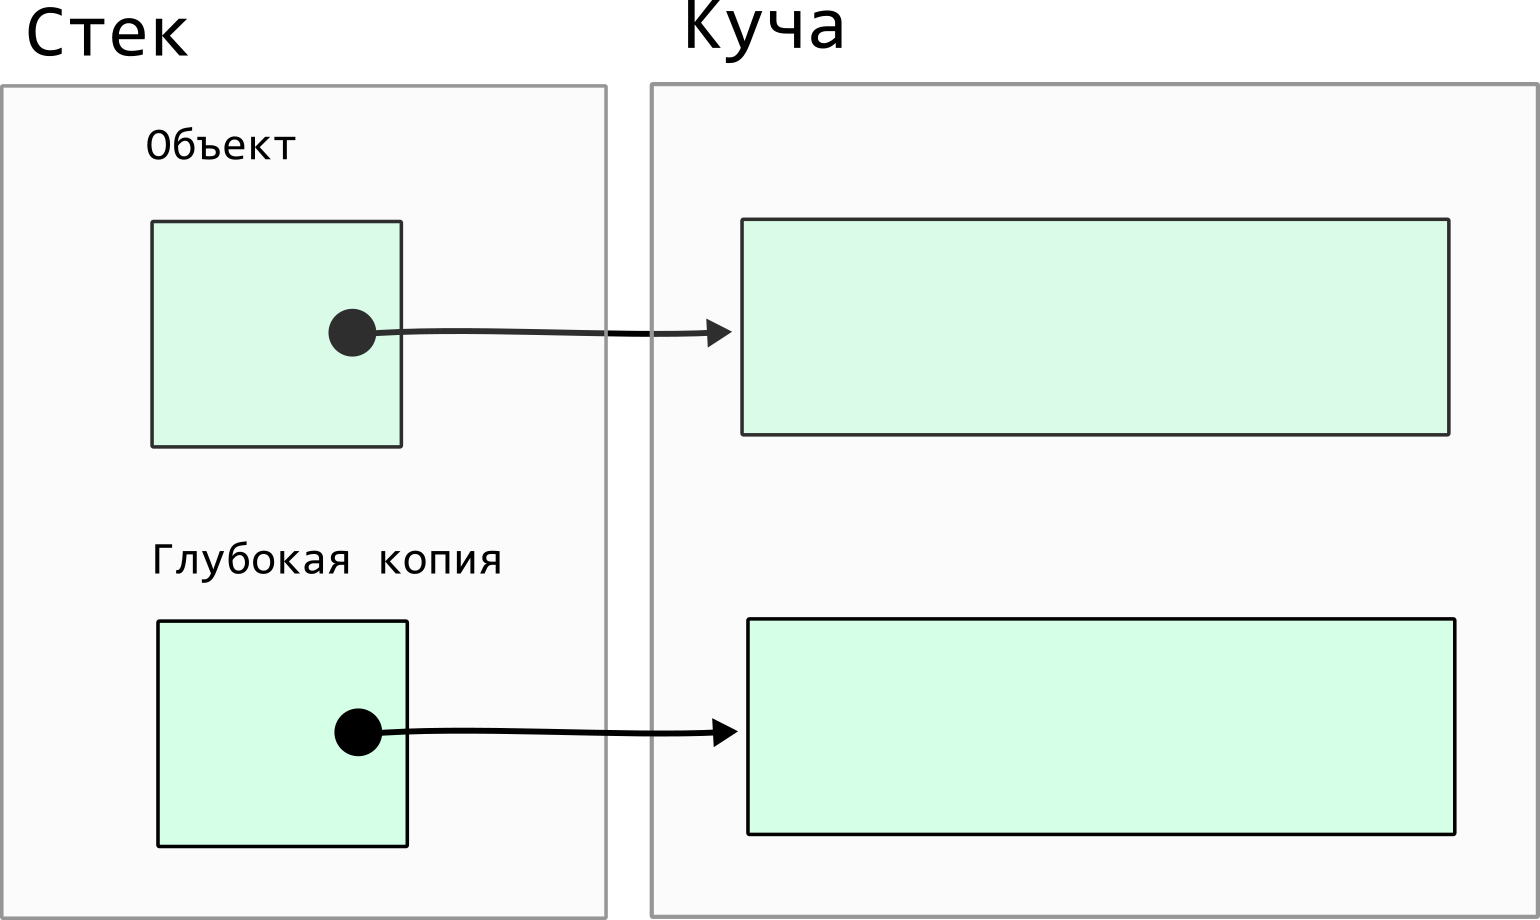
\includegraphics[scale=0.9]{../images/deep.png}
\end{center}

При поверхностном копировании происходит только побайтовое копирование полей объекта. В том числе копируются все указатели, которые продолжают указывать на ту же область памяти в куче. Так, например, работает присваивание структур в языке C.

\begin{center}
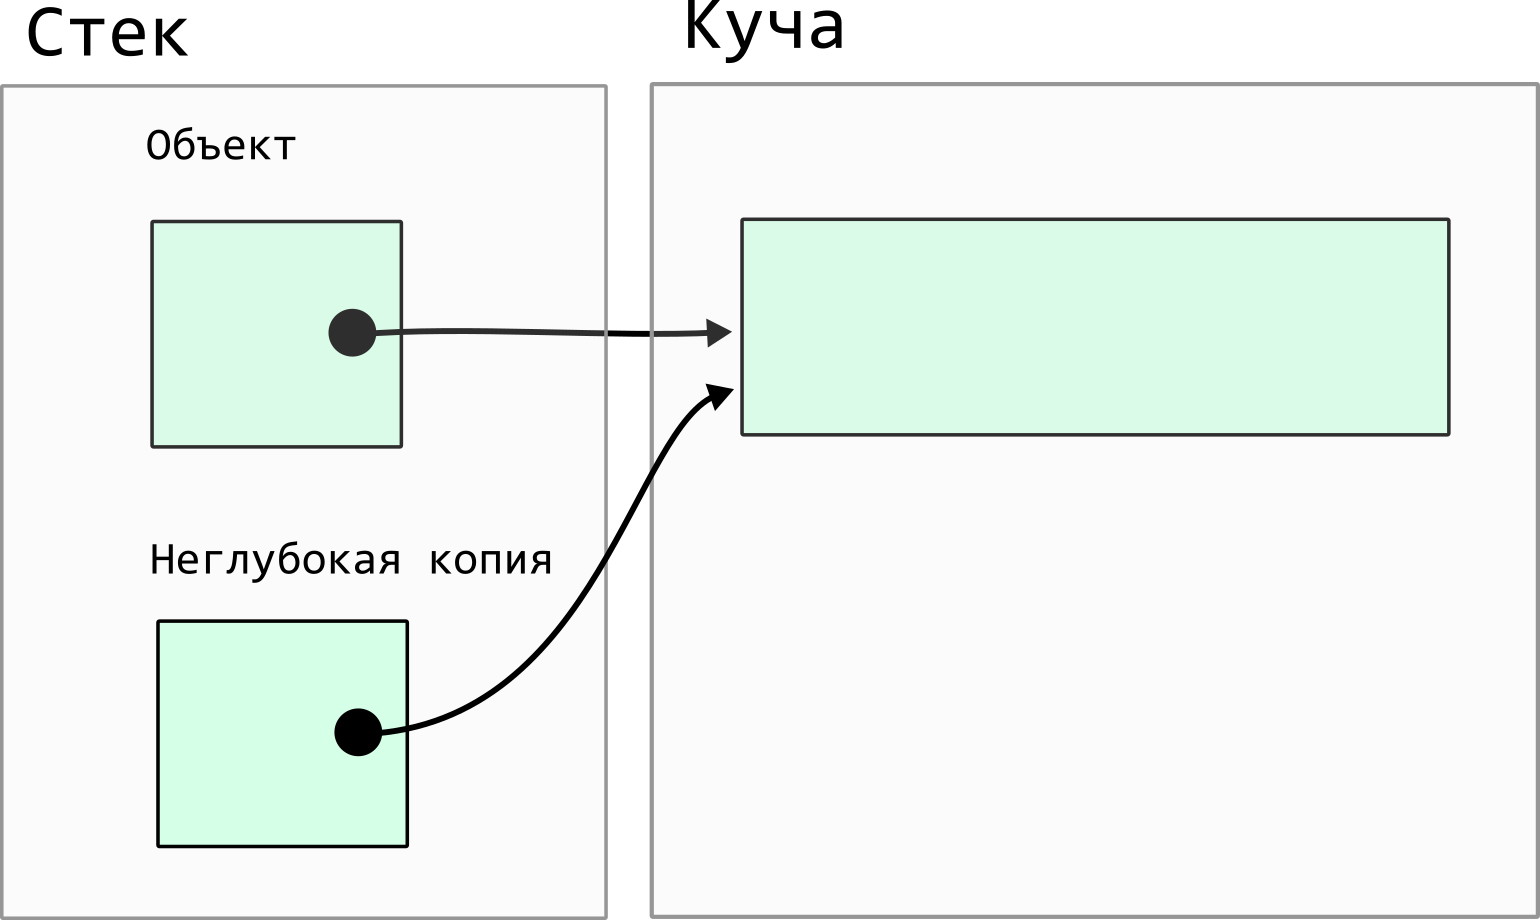
\includegraphics[scale=0.9]{../images/shallow.png}
\end{center}

Поверхностное копирование имеет множество недостатков, связанных с безопастностью работы программы. Более того, иногда нам нужна полная копия объекта и поверхностное копирование просто не подойдёт. Но есть и большое преимущество такого копирования -- оно значительно более эффективно.

\newpage
\section*{Часть 2: Копирование и Перемещение в C++}
\subsection*{Копирование}
Под копированием в языке C++ понимается глубокое копирование.  В примере ниже вектор \texttt{a} копируется в вектор \texttt{b} с помощью конструктора копирования.
\begin{lstlisting}
std::vector<int> a {10, 20, 30, 40};
a.reserve(7);
std::vector<int> b = a;
\end{lstlisting}
\begin{center}
\vspace*{-2.5cm}
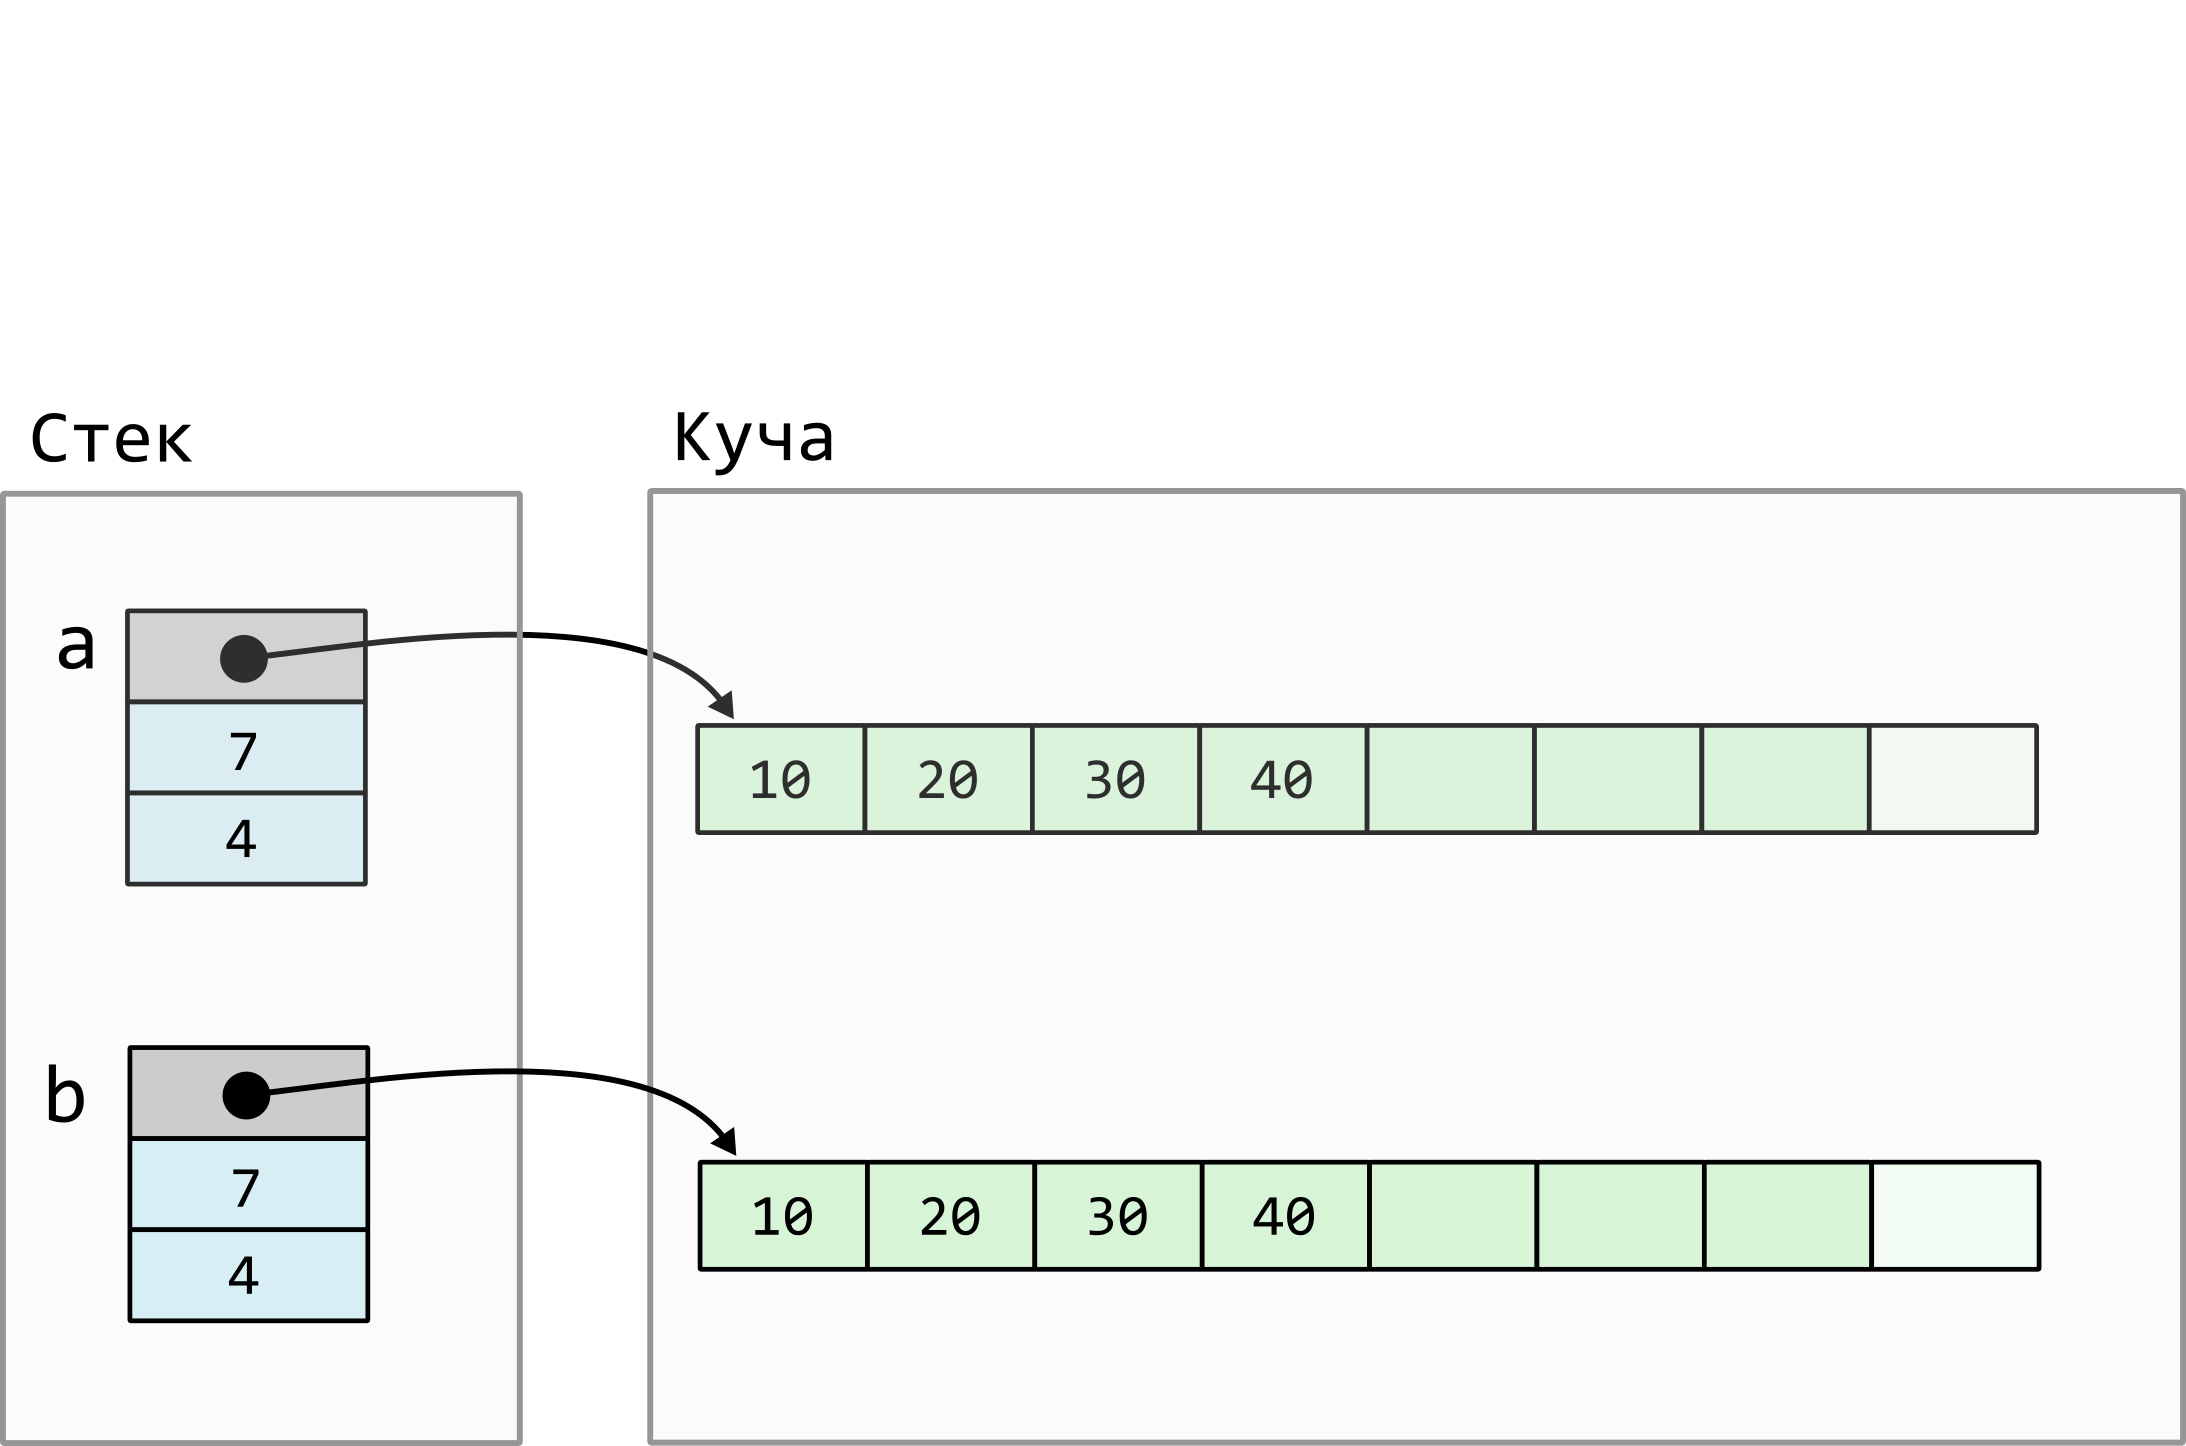
\includegraphics[scale=0.7]{../images/vector_copy.png}
\end{center}

\subsection*{Перемещение}
Под перемещением в C++ понимается операция, состоящая из двух частей:
\begin{enumerate}
\item Поверхностное копирование
\item Изменение объекта, из которого производилась копия. Объект должен перестать владеть ресурсом, но должен находится в корректном состоянии.
\end{enumerate}
Перемещение проводится с помощью специальной стандартной функции \texttt{std::move}. В примере ниже проводится перемещение вектора \texttt{a} в вектор \texttt{b}. При этом вектор \texttt{a} после перемещения не содержит указатель на память в куче. Тем не менее вектор \texttt{a} продолжает находиться в корректном состоянии. В него, например, можно скопировать или переместить другой вектор.

\begin{lstlisting}
std::vector<int> a {10, 20, 30, 40};
a.reserve(7);
std::vector<int> b = std::move(a);
\end{lstlisting}
\begin{center}
\vspace*{-2.5cm}
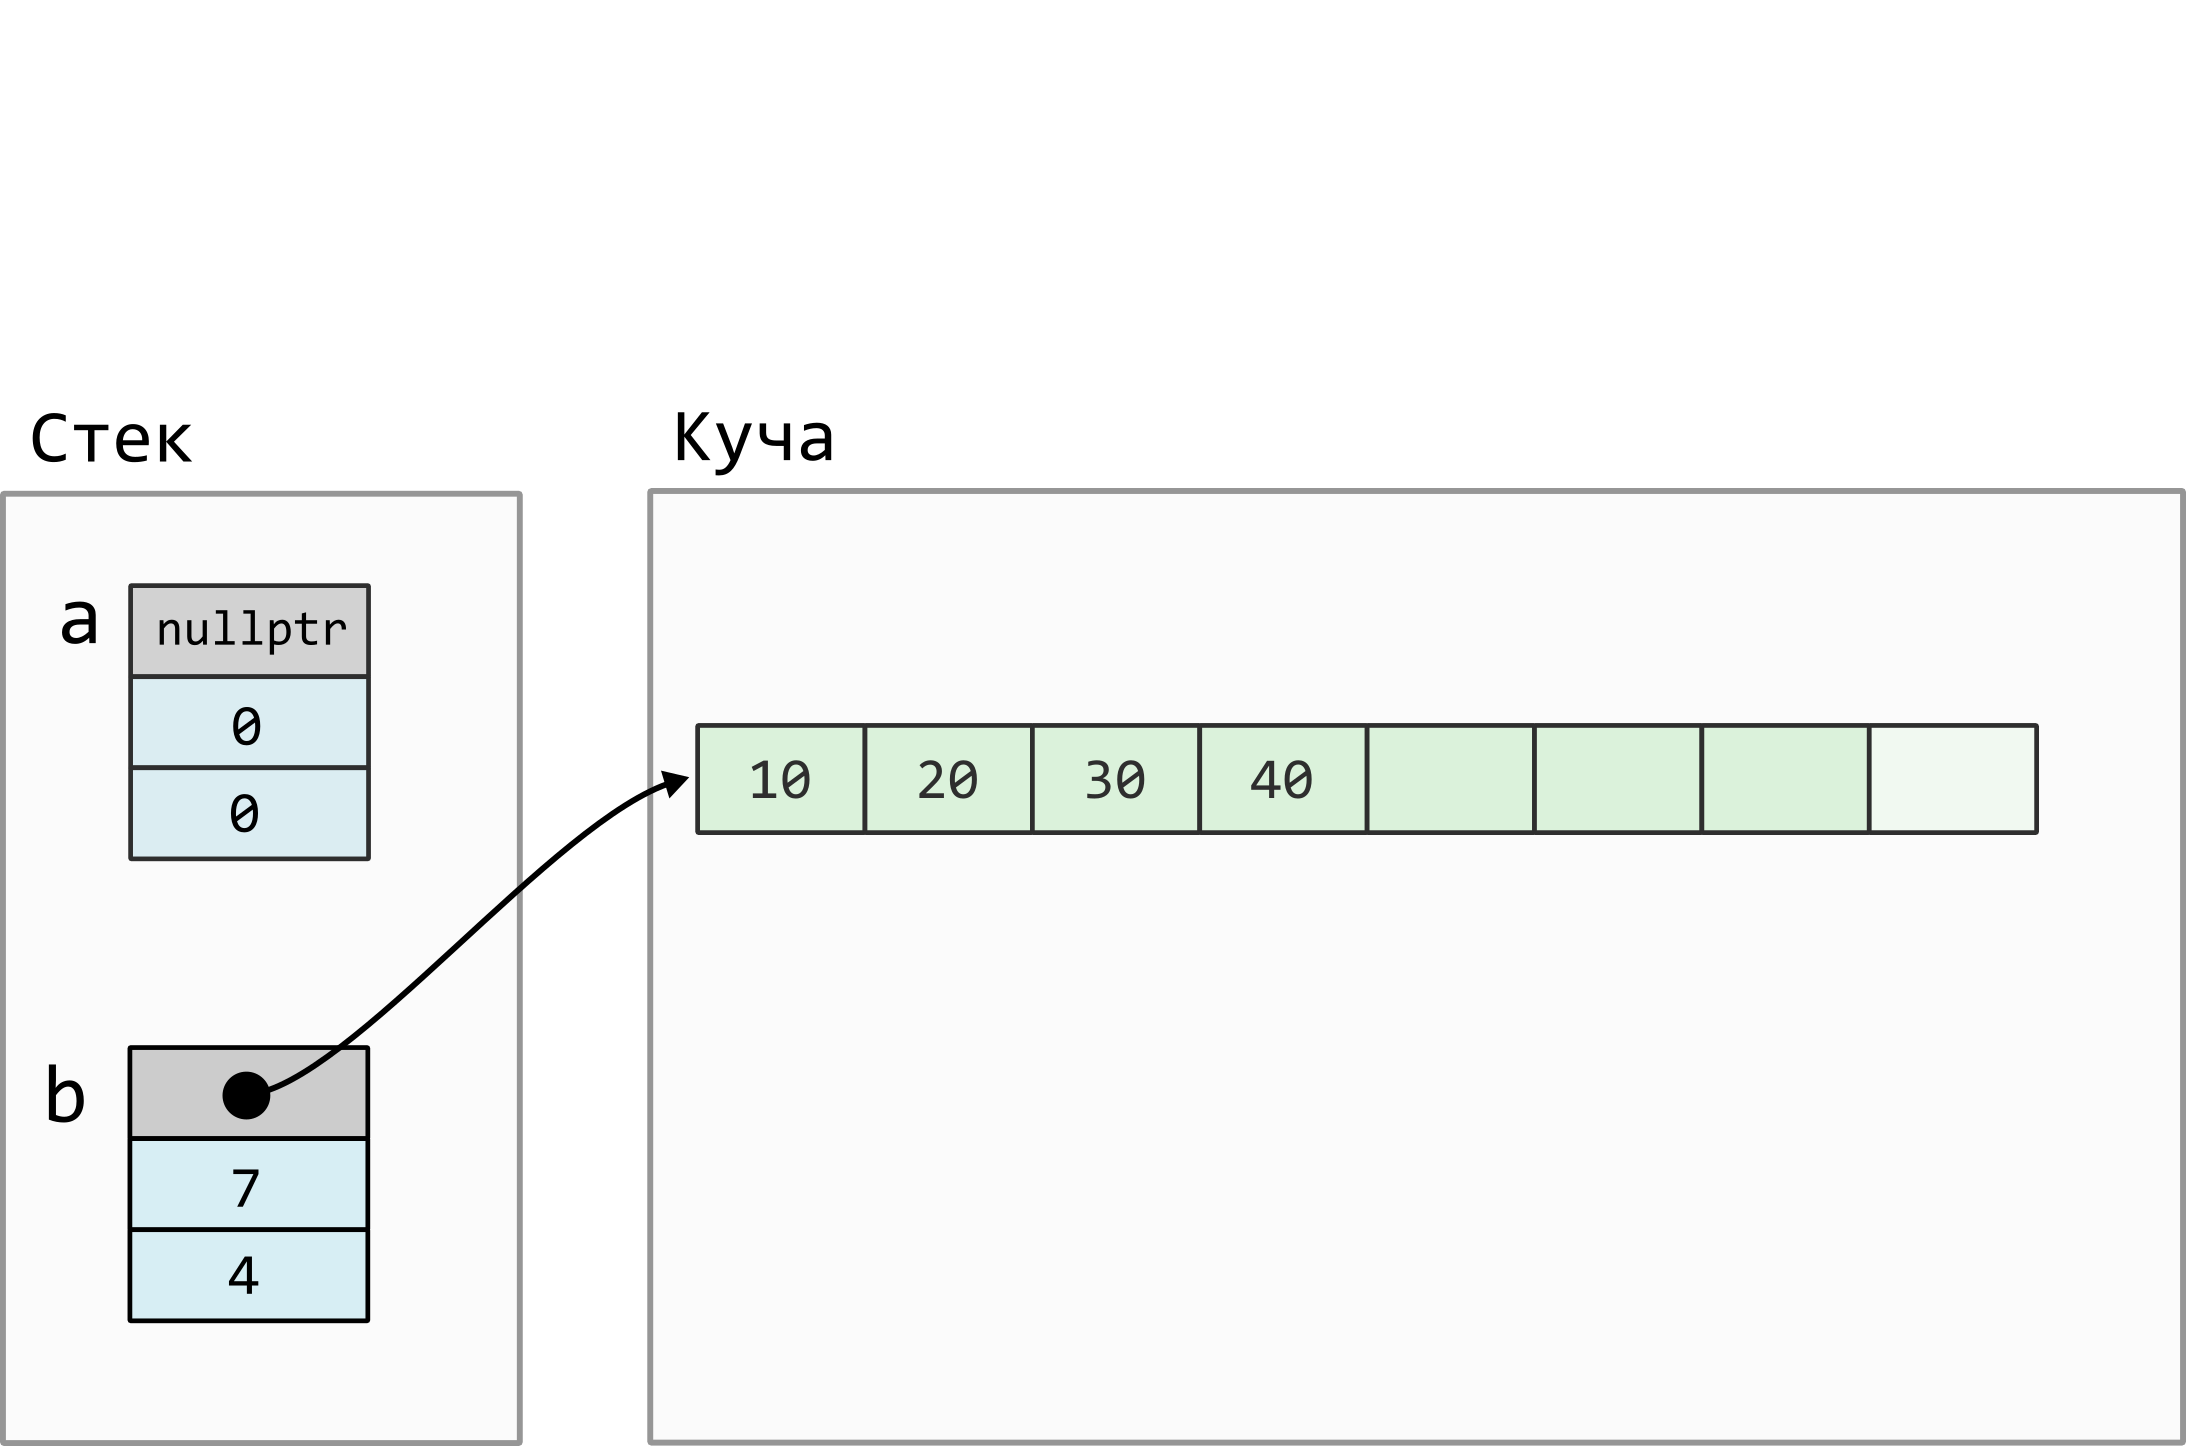
\includegraphics[scale=0.7]{../images/vector_move.png}
\end{center}


\newpage

\subsection*{Польза перемещения}
Перемещение очень полезно тогда, когда объект из которого производится перемещение перестаёт быть нужным после перемещения. В этих случаях перемещение позволяет существенно ускорить программу.
\subsubsection*{Перемещение временных объектов}
Рассмотрим следующий пример. Есть две строки \texttt{s1} и \texttt{s2}, которые потенциально могут быть очень длинными. Мы хотим конкатенировать эти строки и сохранить результат в другой строке \texttt{s}.
\begin{lstlisting}
s = s1 + s2;
\end{lstlisting}
В этом случае будут произведены следующие операции:
\begin{enumerate}
\item Конкатенирование строки с помощью метода \texttt{operator+} строки. При этом создаётся некоторый временный объект (типа \texttt{std::string}), в котором будет хранится результат конкатенации.
\item Перемещение этого временного объекта в строку \texttt{s}.
\end{enumerate}
Без перемещения, на втором шаге нам бы пришлось копировать временный объект в строку \texttt{s}, что было бы намного менее эффективно.
Аналогично, перемещение ускоряет программу, когда мы передаём временные объект в функции по значению.
\begin{lstlisting}
void func(std::string s) {...};
// ...
func(s1 + s2); // Тут используется
\end{lstlisting}

\subsubsection*{Ускорение некоторых операций с помощью перемещения}
Перемещение может быть полезно не только для временных объектов. Перемещая обычные невременные объекты можно ускорить многие алгоритмы. Рассмотрим, например, задачу обмена значений двух строк, которые потенциально могут быть очень длинными:
\begin{lstlisting}
std::swap(s1, s2);
\end{lstlisting}
Функция \texttt{swap} просто перемещает объекты и реализована следующим образом:
\begin{lstlisting}
template<typename T> 
void swap(T& a, T& b) 
{
    T temp = std::move(a);
    a = std::move(b);
    b = std::move(temp);
}
\end{lstlisting}
Без перемещения объекты пришлось бы многократно копировать внутри функции \texttt{swap}, что было бы очень неэффективно для объектов, владеющих памятью в куче. С перемещением \texttt{swap} работает намного быстрее для объектов, выделяющих память в куче. Соответственно, будут работать намного быстрее все алгоритмы, использующие \texttt{swap} (например, алгоритмы сортировки).

\subsubsection*{Возвращаемое значение функции}
Перемещение может помочь при возврате объекта из функции. Но в этом случае нет необходимости использовать \texttt{std::move}, так как перемещение происходит автоматически. Более того, использование \texttt{std::move} может не дать компилятору использовать RVO(Return Value Optimization), что может привести к более медленному коду.


\newpage
\section*{Часть 3: \texttt{lvalue} и \texttt{rvalue}}


\newpage

Для объекта можно написать конструктор копирования и оператор присваивания, которые должны производить глубокое копирование объекта. По аналогии с копированием, для объекта можно создать конструктор перемещения и оператор присваивания перемещением.
\end{document}